\documentclass[11pt,letterpaper]{article}
\usepackage[utf8]{inputenc}
\usepackage[T1]{fontenc}
\usepackage[spanish]{babel}
\usepackage{amsmath}
\usepackage{amsfonts}
\usepackage{amssymb}
\usepackage{graphicx}
\usepackage{lmodern}
\usepackage{xspace}
\usepackage{multicol}
\usepackage{hyperref}
\usepackage{float}
\usepackage{hyperref}
\usepackage{color}
\usepackage{framed}



\usepackage[left=2cm,right=2cm,top=2cm,bottom=2cm]{geometry}

\newcommand{\X}{\mathbb{X}}
\newcommand{\x}{\mathbf{x}}
\newcommand{\Y}{\mathbf{Y}}
\newcommand{\y}{\mathbf{y}}
\newcommand{\xbarn}{\bar{x}_n}
\newcommand{\ybarn}{\bar{y}_n}
\newcommand{\paren}[1]{\left( #1 \right)}
\newcommand{\llaves}[1]{\left\lbrace #1 \right\rbrace}
\newcommand{\barra}{\,\vert\,}
\newcommand{\mP}{\mathbb{P}}
\newcommand{\mE}{\mathbb{E}}
\newcommand{\mR}{\mathbb{R}}
\newcommand{\mJ}{\mathbf{J}}
\newcommand{\mX}{\mathbf{X}}
\newcommand{\mS}{\mathbf{S}}
\newcommand{\mA}{\mathbf{A}}
\newcommand{\unos}{\boldsymbol{1}}
\newcommand{\xbarnv}{\bar{\mathbf{x}}_n}
\newcommand{\abs}[1]{\left\vert #1 \right\vert}
\newcommand{\muv}{\boldsymbol{\mu}}
\newcommand{\mcov}{\boldsymbol{\Sigma}}
\newcommand{\vbet}{\boldsymbol{\beta}}
\newcommand{\veps}{\boldsymbol{\epsilon}}
\newcommand{\mcC}{\mathcal{C}}
\newcommand{\mcR}{\mathcal{R}}
\newcommand{\mcN}{\mathcal{N}}

\newcommand{\ceros}{\boldsymbol{0}}
\newcommand{\mH}{\mathbf{H}}
\newcommand{\ve}{\mathbf{e}}
\newcommand{\avec}{\mathbf{a}}
\newcommand{\res}{\textbf{RESPUESTA}\\}

\newcommand{\defi}[3]{\textbf{Definición:#3}}
\newcommand{\fin}{$\blacksquare.$}
\newcommand{\finf}{\blacksquare.}
\newcommand{\tr}{\text{tr}}
\newcommand*{\temp}{\multicolumn{1}{r|}{}}

\newcommand{\grstep}[2][\relax]{%
   \ensuremath{\mathrel{
       {\mathop{\longrightarrow}\limits^{#2\mathstrut}_{
                                     \begin{subarray}{l} #1 \end{subarray}}}}}}
\newcommand{\swap}{\leftrightarrow}

\newcommand{\gen}{\text{gen}}
\newtheorem{thmt}{Teorema:}
\newtheorem{thmd}{Definición:}
\newtheorem{thml}{Lema:}

\begin{document}
\begin{table}[ht]
\centering
\begin{tabular}{c}
\textbf{Maestría en Computo Estadístico}\\
\textbf{Optimización} \\
\textbf{Tarea de Programación Lineal}\\
\today \\
\emph{Enrique Santibáñez Cortés}\\
Repositorio de Git: \href{https://https://github.com/Enriquesec/Optimizacion/tree/master/tareas/tarea_1}{Tarea 1}.
\end{tabular}
\end{table}

\section{Método gráfico}

\begin{enumerate}
\item Obteneer la solución optima (si existe) del siguiente problema:
\begin{align*}
\max\ \ \ \ & z=3x_1+3x_2\\
s.a:\ \ \ \ & x_1-2x_2 \leq 2\\
	 & -2x_1+x_2\leq 2\\
	 &x_1,x_2 \geq 0
\end{align*}

\res Gráficamos cada una de las restricciones (ver Figura \ref{ejercicio_1}). El área roja representa la región factible que cumplen todas las restricciones, \textbf{entonces como queremos maximizar y el área no esta acotada podemos concluir que no existe una solución óptima.}

\begin{figure}[H] \label{ejercicio_1}
\centering
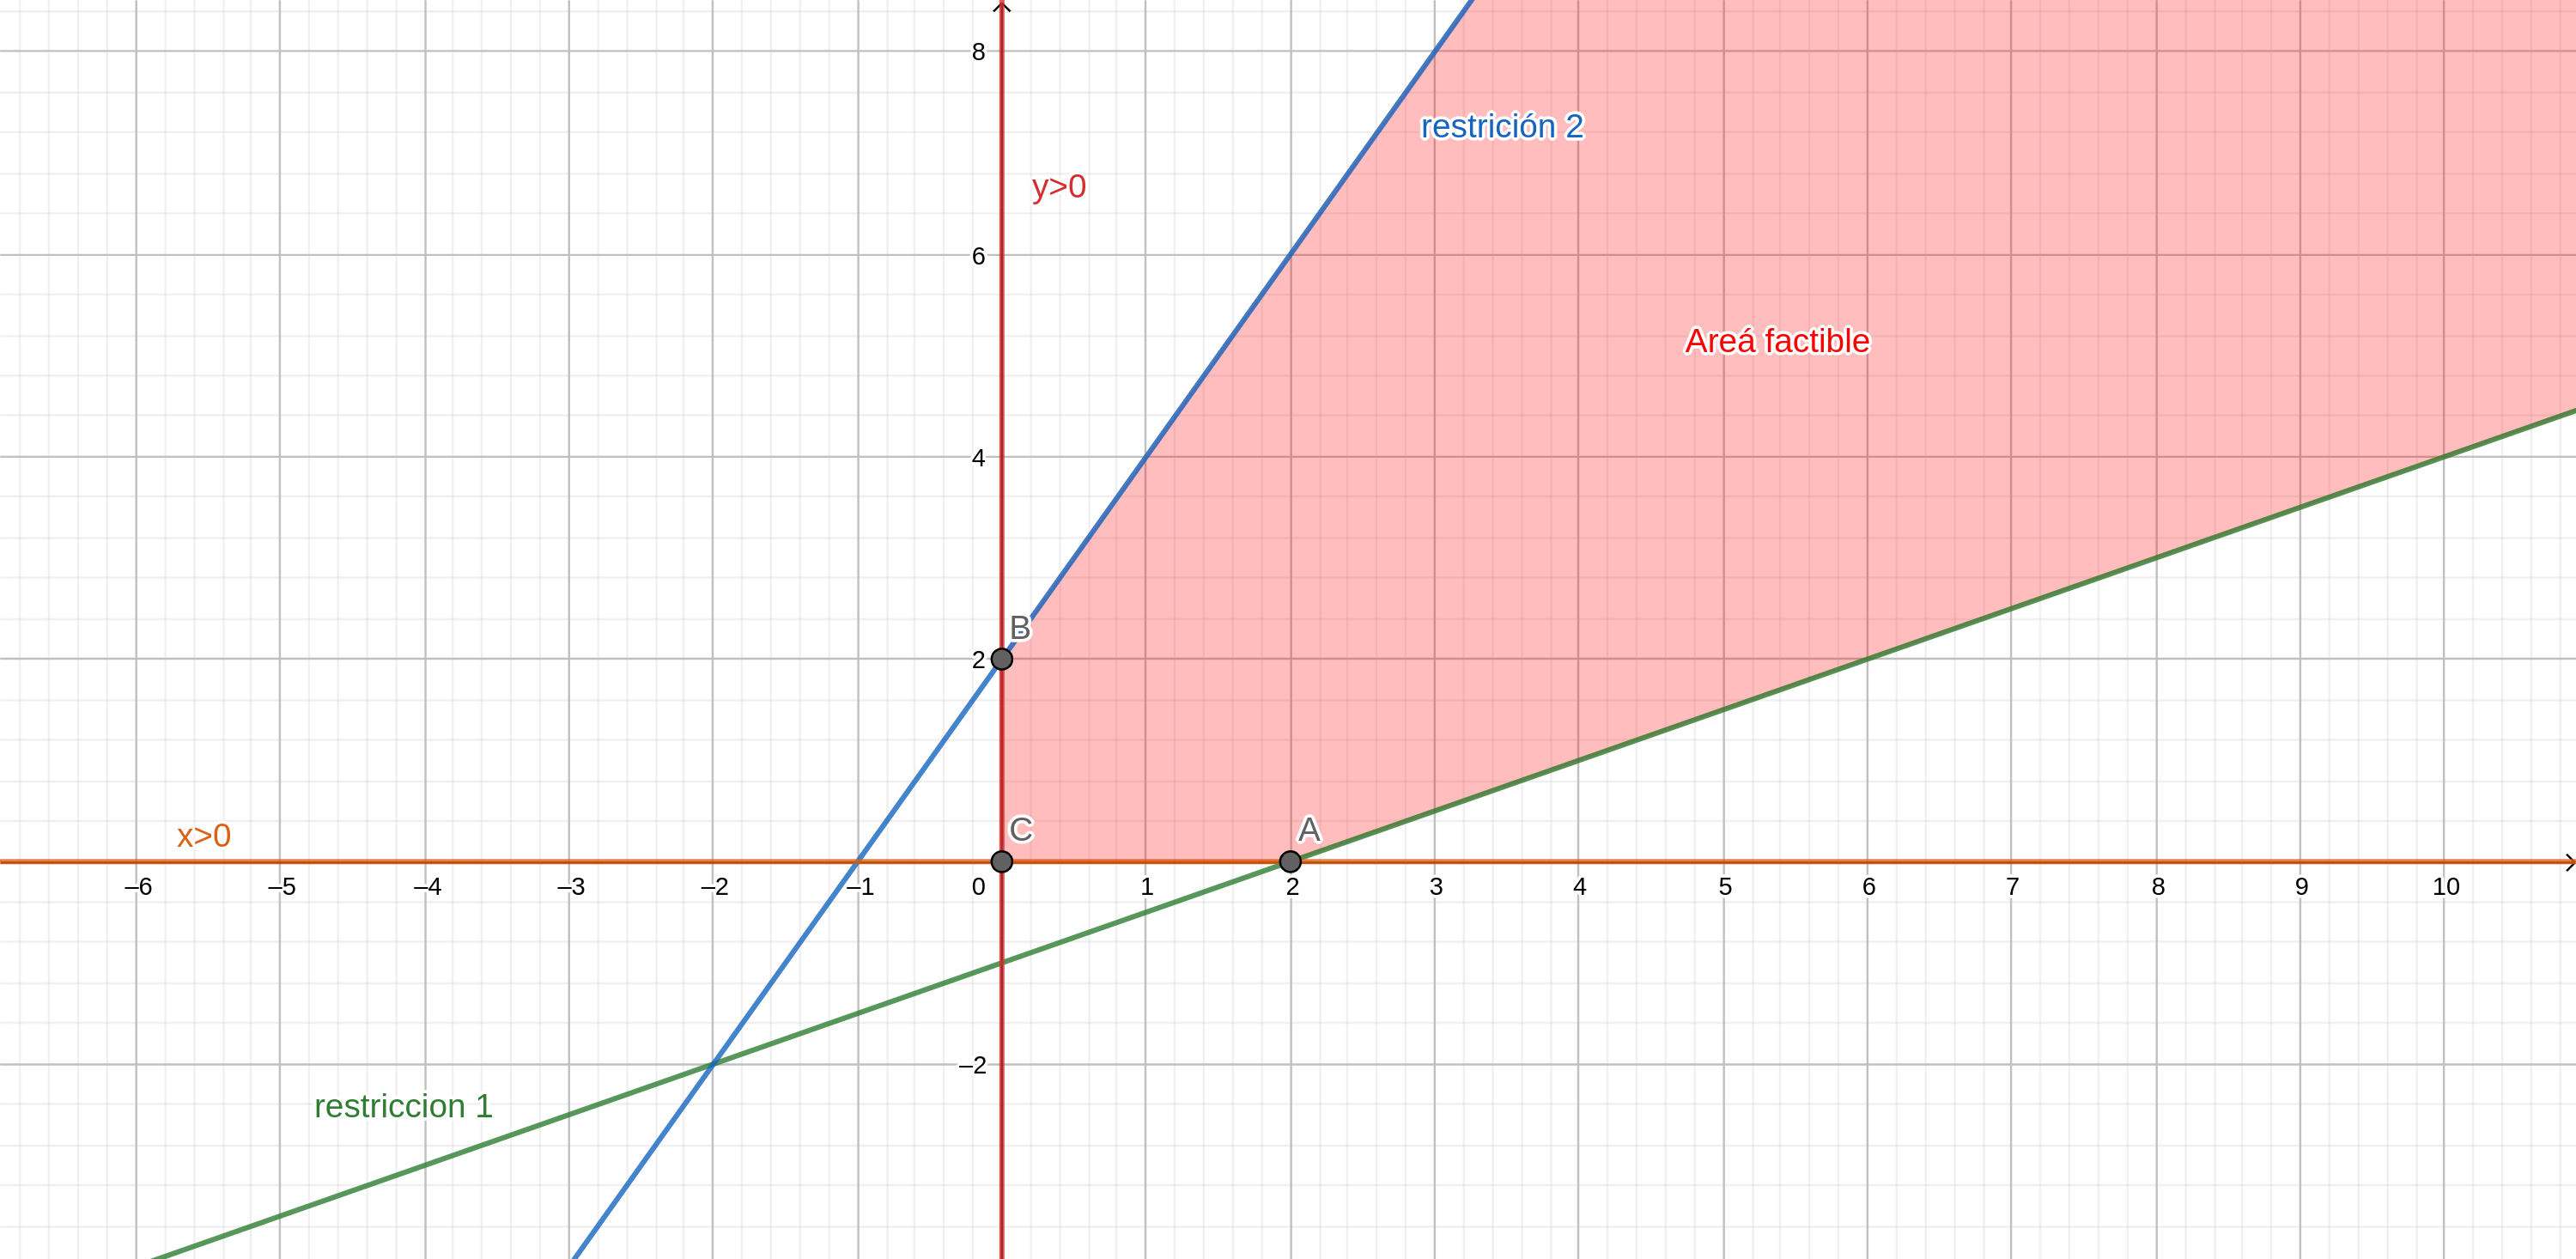
\includegraphics[scale=0.7]{ejercicio_1.png}
\caption{Representación grafica de las restricciones.}
\end{figure}

\section{Modelación matemática y método simplex:}

\item La compañía ANCE, S.A., produce una línea de artículos de peltre para uso casero, la cual consta de varios productos. El sistema de manufactura se divide en varios departamentos: cortado, troquelado y esmaltado. Cada artículo tiene una utilidad unitaria diferente. A continuación se presenta la información relevante. Formular este problema considerando que la compañía desea maximizar la utilidad total.
\begin{table}[H]
\centering
\begin{tabular}{c|c|c|c|c|c}
Departamento (operación) & Artículo 1 & Artículo 2 & Artículo 3 & Artículo 4 & Capacidad productiva\\ \hline \hline 
Cortado & 10 & 20 & 2 & 3 & 4000\\
Troquelado & 5 & 5 & 5 & 4 & 1500\\
Esmaltado & 4 & 2 & 6 & 6 & 800\\
Utilidad unitaria $(\$)$ & 10 & 15 & 4 & 2&  \\ \hline \hline
\end{tabular}
\caption{Índice de producción (unidades/hora)}
\end{table}
En la modelación declare a $z$ como la función objetivo y considere las siguientes variables de decisión:
\begin{table}[H]
\begin{tabular}{c}
$x_1$: cantidad del artículo 1\\
$x_2$: cantidad del artículo 2\\
$x_3$: cantidad del artículo 3\\
$x_4$: cantidad del artículo 4
\end{tabular}
\end{table}

\res El objetivo que tiene la compañía es maximizar la utilidad total, entonces ocupando la utiliad unitaria de cada artículo tenemos que la función objetivo es:
\begin{align*}
\max\ \ \ \ & z=10x_1+15x_2+4x_3+2x_4.\\
\end{align*}
Ahora, considerando la capacidad productiva como el límite de $horas\_de\_operación/periodo$ que tiene cada departamento, podemos traducir esta capacidad como la restrición, es decir,
\begin{align*}
s.a:\ \ \ \ & 10x_1+20x_2 +2x_3+3x_4\leq 4000\\
	 & 5x_1+5x_2+5x_3+4x_4\leq 1500\\
	 & 4x_1+2x_2+6x_3+6x_4 \leq 800\\
	 & x_1,x_2,x_3,x_4 \geq 0. 
\end{align*}
Ahora, no sabemos específicamente si los artículos no pueden ser entero o no. Pero si no es posible tener una fración del $x_i \ \i=1,\cdots, 4$ entonces tenemos que agregar la restricción:
\begin{align*}
s.a:\ \ \ \ & x_1,x_2,x_3, x_4\in \mathbb{N}.
\end{align*}
De caso contrario no sería necesarion agregar esta restricción. \ \ \ \ \fin

\item Considerar la relajación lineal del modelo del problema 2. Resolver el modelo obtenido con el método simplex tabular.

\res Como estabamos considerando la relajación lineal, esto significa que no agreguemos la restricción de que los productos no son enteros, entonces el problema a resolver es:
\begin{align*}
\max\ \ \ \ & z=10x_1+15x_2+4x_3+2x_4.\\
s.a:\ \ \ \ & 10x_1+20x_2 +2x_3+3x_4\leq 4000\\
	 & 5x_1+5x_2+5x_3+4x_4\leq 1500\\
	 &  4x_1+2x_2+6x_3+6x_4 \leq 800\\
	 & x_1,x_2,x_3,x_4 \geq 0. 
\end{align*}
Primero pasamos el problema a la forma estádar, para ello agregamos las variables de holgura $x_5, x_6$ y $x_7$
\begin{align*}
\max\ \ \ \ & z=10x_1+15x_2+4x_3+2x_4+0x_5+0x_6+0x_7.\\
s.a:\ \ \ \ & 10x_1+20x_2 +2x_3+3x_4+x_5 = 4000\\
	 & 5x_1+5x_2+5x_3+4x_4+x_6= 1500\\
	 &  4x_1+2x_2+6x_3+6x_4  +x_7= 800\\
	 & x_1,x_2, x_3, x_4, x_5,x_6,x_7 \geq 0. 
\end{align*}
Ahora reescribimos la función objetivo como 
\begin{align*}
-z+10x_1+15x_2+4x_3+2x_4+0x_5+0x_6+0x_7=0.
\end{align*}
Por lo que la tabla simplex sería:
\begin{equation}
\begin{array}{c}
\\
z \\ 
x_5 \\
x_6 \\
x_7 
\end{array}
\begin{bmatrix}
\begin{array}{c||cccccccc}
  z & x_1 & x_2 & x_3 & x_4 & x_5 & x_6 & x_7 & LD \\ \hline \hline
  1 &-10 &-15 &-4 &-2 & 0 & 0 & 0 & 0\\ 
  0 & 10 & 20 & 2 & 3 & 1 & 0 & 0 & 4000  \\
  0 &  5 &  5 & 5 & 4 & 0 & 1 & 0 & 1500 \\
  0 &  4 &  2 & 6 & 6 & 0 & 0 & 1 & 800 \\
\end{array}
\end{bmatrix}
\end{equation}
Veamos que no se cumple la prueba de optimalidad, la cual es que todos los coeficientes de la primer fila deben de ser $\geq 0$. La variable que entra es $x_2$, ya que tiene el coeficiente más negativo. Y la variable que sale de la base es $x_5$, ya que $\min\left\{\frac{4000}{20} ,\frac{15000}{5},\frac{800}{2}\right\}= 200.$ Entonces
\begin{equation}
\begin{array}{c}
\\
z \\ 
x_2 \\
x_6 \\
x_7
\end{array}
\begin{bmatrix}
\begin{array}{c||cccccccc}
  z & x_1 & x_2 & x_3 & x_4 & x_5 & x_6 & x_7 & LD\\ \hline \hline
  1 &-10 &-15 &-4 &-2 & 0 & 0 & 0 & 0\\ 
  0 & 1/2 & 1 & 1/10 & 3/20 & 1/20 & 0 & 0 & 200  \\
  0 &  5 &  5 & 5 & 4 & 0 & 1 & 0 & 1500 \\
  0 &  4 &  2 & 6 & 6 & 0 & 0 & 1 & 800 \\
\end{array}
\end{bmatrix}
\end{equation}
Transformamos a $x_2$ en su forma canónica
\begin{equation}
\begin{array}{c}
\\
z \\ 
x_2 \\
x_6 \\
x_7
\end{array}
\begin{bmatrix}
\begin{array}{c||cccccccc}
  z & x_1 & x_2 & x_3 & x_4 & x_5 & x_6 & x_7 & LD\\ \hline \hline
  1 &-5/2 & 0 &-5/2 &1/4 & 3/4 & 0 & 0 & 3000\\ 
  0 & 1/2 & 1 & 1/10 & 3/20 & 1/20 & 0 & 0 & 200  \\
  0 &  5/2 &  0 & 9/5 & 13/4 & -1/4 & 1 & 0 & 500 \\
  0 &  3 &  0 & 29/5 & 57/10 & -1/10 & 0 & 1 & 400 \\
\end{array}
\end{bmatrix}
\end{equation}
Vemos que no se cumple la prueba de optimalidad: ya que no todos los elementos de la primer fila son $\geq 0$. Entonces la nueva variable que entra es $x_1$ y la variable que sale de la base es $x_7$, ya que $\min\left\{400 ,\frac{15000}{5},\frac{800}{4}\right\}= 200.$ Entonces
\begin{equation}
\begin{array}{c}
\\
z \\ 
x_2 \\
x_6 \\
x_1
\end{array}
\begin{bmatrix}
\begin{array}{c||cccccccc}
  z & x_1 & x_2 & x_3 & x_4 & x_5 & x_6 & x_7 & LD\\ \hline \hline
  1 &-5/2 & 0 &-5/2 &1/4 & 3/4 & 0 & 0 & 3000\\ 
  0 & 1/2 & 1 & 1/10 & 3/20 & 1/20 & 0 & 0 & 200  \\
  0 &  5/2 &  0 & 9/5 & 13/4 & -1/4 & 1 & 0 & 500 \\
  0 &  1 &  0 & 29/15 & 19/10 & -1/30 & 0 & 1/3 & 400/3 \\
\end{array}
\end{bmatrix}
\end{equation}
Transformamos a $x_1$ en su forma canónica
\begin{equation} \label{t_optima_original}
\begin{array}{c}
\\
z \\ 
x_2 \\
x_6 \\
x_1
\end{array}
\begin{bmatrix}
\begin{array}{c||cccccccc}
  z & x_1 & x_2 & x_3 & x_4 & x_5 & x_6 & x_7 & LD\\ \hline \hline
  1 & 0 & 0 & 7/3 & 5 & 2/3 & 0 & 5/6 & 10000/3\\ 
  0 & 0 & 1 &-13/15 & -4/5 & 1/15 & 0 &-1/6 & 400/3  \\
  0 & 0 & 0 &-1/3 & -3/2 & -1/6 & 1 & -5/6& 500/3 \\
  0 & 1 & 0 & 29/15 & 19/10 & -1/30 & 0 & 1/3 & 400/3 \\
\end{array}
\end{bmatrix}
\end{equation}
Usando la prueba de óptimalidad, \textbf{podemos conclluir que ya llegamos la solución óptima. La cual es $x^* = \begin{pmatrix}
400/3 & 400/3 & 0 & 0
\end{pmatrix}$ y el valor de la función objetivo es $z^*=10000/3$} \ \ \ \ \fin

\section{Dualidad}

\item Encontrar el modelo  dual del problema 1 y encontrar la solución con el método gráfico.

\res \begin{framed}
    \begin{thmd} \label{d_dual}
	(Visto en clase, pag. 45) Problemas de programación lineal de maximizar y minimizar pueden ser representados como:
	\begin{align*}
	\min\ \ \ \ & \bf z=c^T \x &  \max\ \ \ \ & w=b^Ty\\
	s.a\ \ \ \ & Ax\geq b &  s.a\ \ \ \ & A^T y\leq c\\
	& x\geq 0 & &  y\geq 0.
	\end{align*}
    \end{thmd}
\end{framed}
\begin{framed}
    \begin{thmt} \label{t_dual_debil}
	(Visto en clase, pag. 52) Si $\x$ y $\mathbf{y}$ son soluciones factibles a los problemas primal y dual, respectivamente; entonces, $\mathbf{c}^T \x \geq \mathbf{b}^T \mathbf{y}$.
	\begin{itemize}
	\item Si cualquiera de los problemas primal y dual es no acotado, entonces el otro no tiene solución factible.
	\item Si $\x*$ y $\mathbf{y}*$  son soluciones factibles a los problemas primal y dual, respectivamente, y $\bf c^T x*=b^Ty*$, entonces son las soluciones ótimas al par de problemas. 
	\end{itemize}
    \end{thmt}
\end{framed}


Primero obtenemos el dual del problema 1, para ello ocupemos la definición \ref{d_dual}. Tenemos que 
\begin{align*}
c=\begin{pmatrix}
3 \\ 3
\end{pmatrix} , \ \ A=\begin{pmatrix}
1 & -2 \\
-2 & 2
\end{pmatrix} \ \ \ \text{y} \ \ \ b=\begin{pmatrix}
2\\
2
\end{pmatrix}.
\end{align*}
Por lo tanto, el problema dual sería
\begin{align*}
\min \ \ \ \ & w=2y_1+2y_2\\
s.a:\ \ \ \ & y_1-2y_2 \geq 3\\
	 & -2y_1+y_2\geq 3\\
	 &y_1,y_2 \geq 0
\end{align*}

Ahora, gráficamos cada una de las restricciones (ver Figura \ref{ejercicio_4}). Las áreas azules representa la región que cumple la resctrición $y_1-2y_2\geq 3 \& y_1\geq 0$, $-2y_1+y_2\geq 3 \& y_2\geq 0$, por lo que se observa que no hay ningún punto que cumpla ambas restriciones al mismo tiempo, \textbf{por lo  que podemos concluir que no hay solución factible.} Esta conclusión tiene sentido con el Teorema (\ref{t_dual_debil}).

\begin{figure}[H] \label{ejercicio_4}
\centering
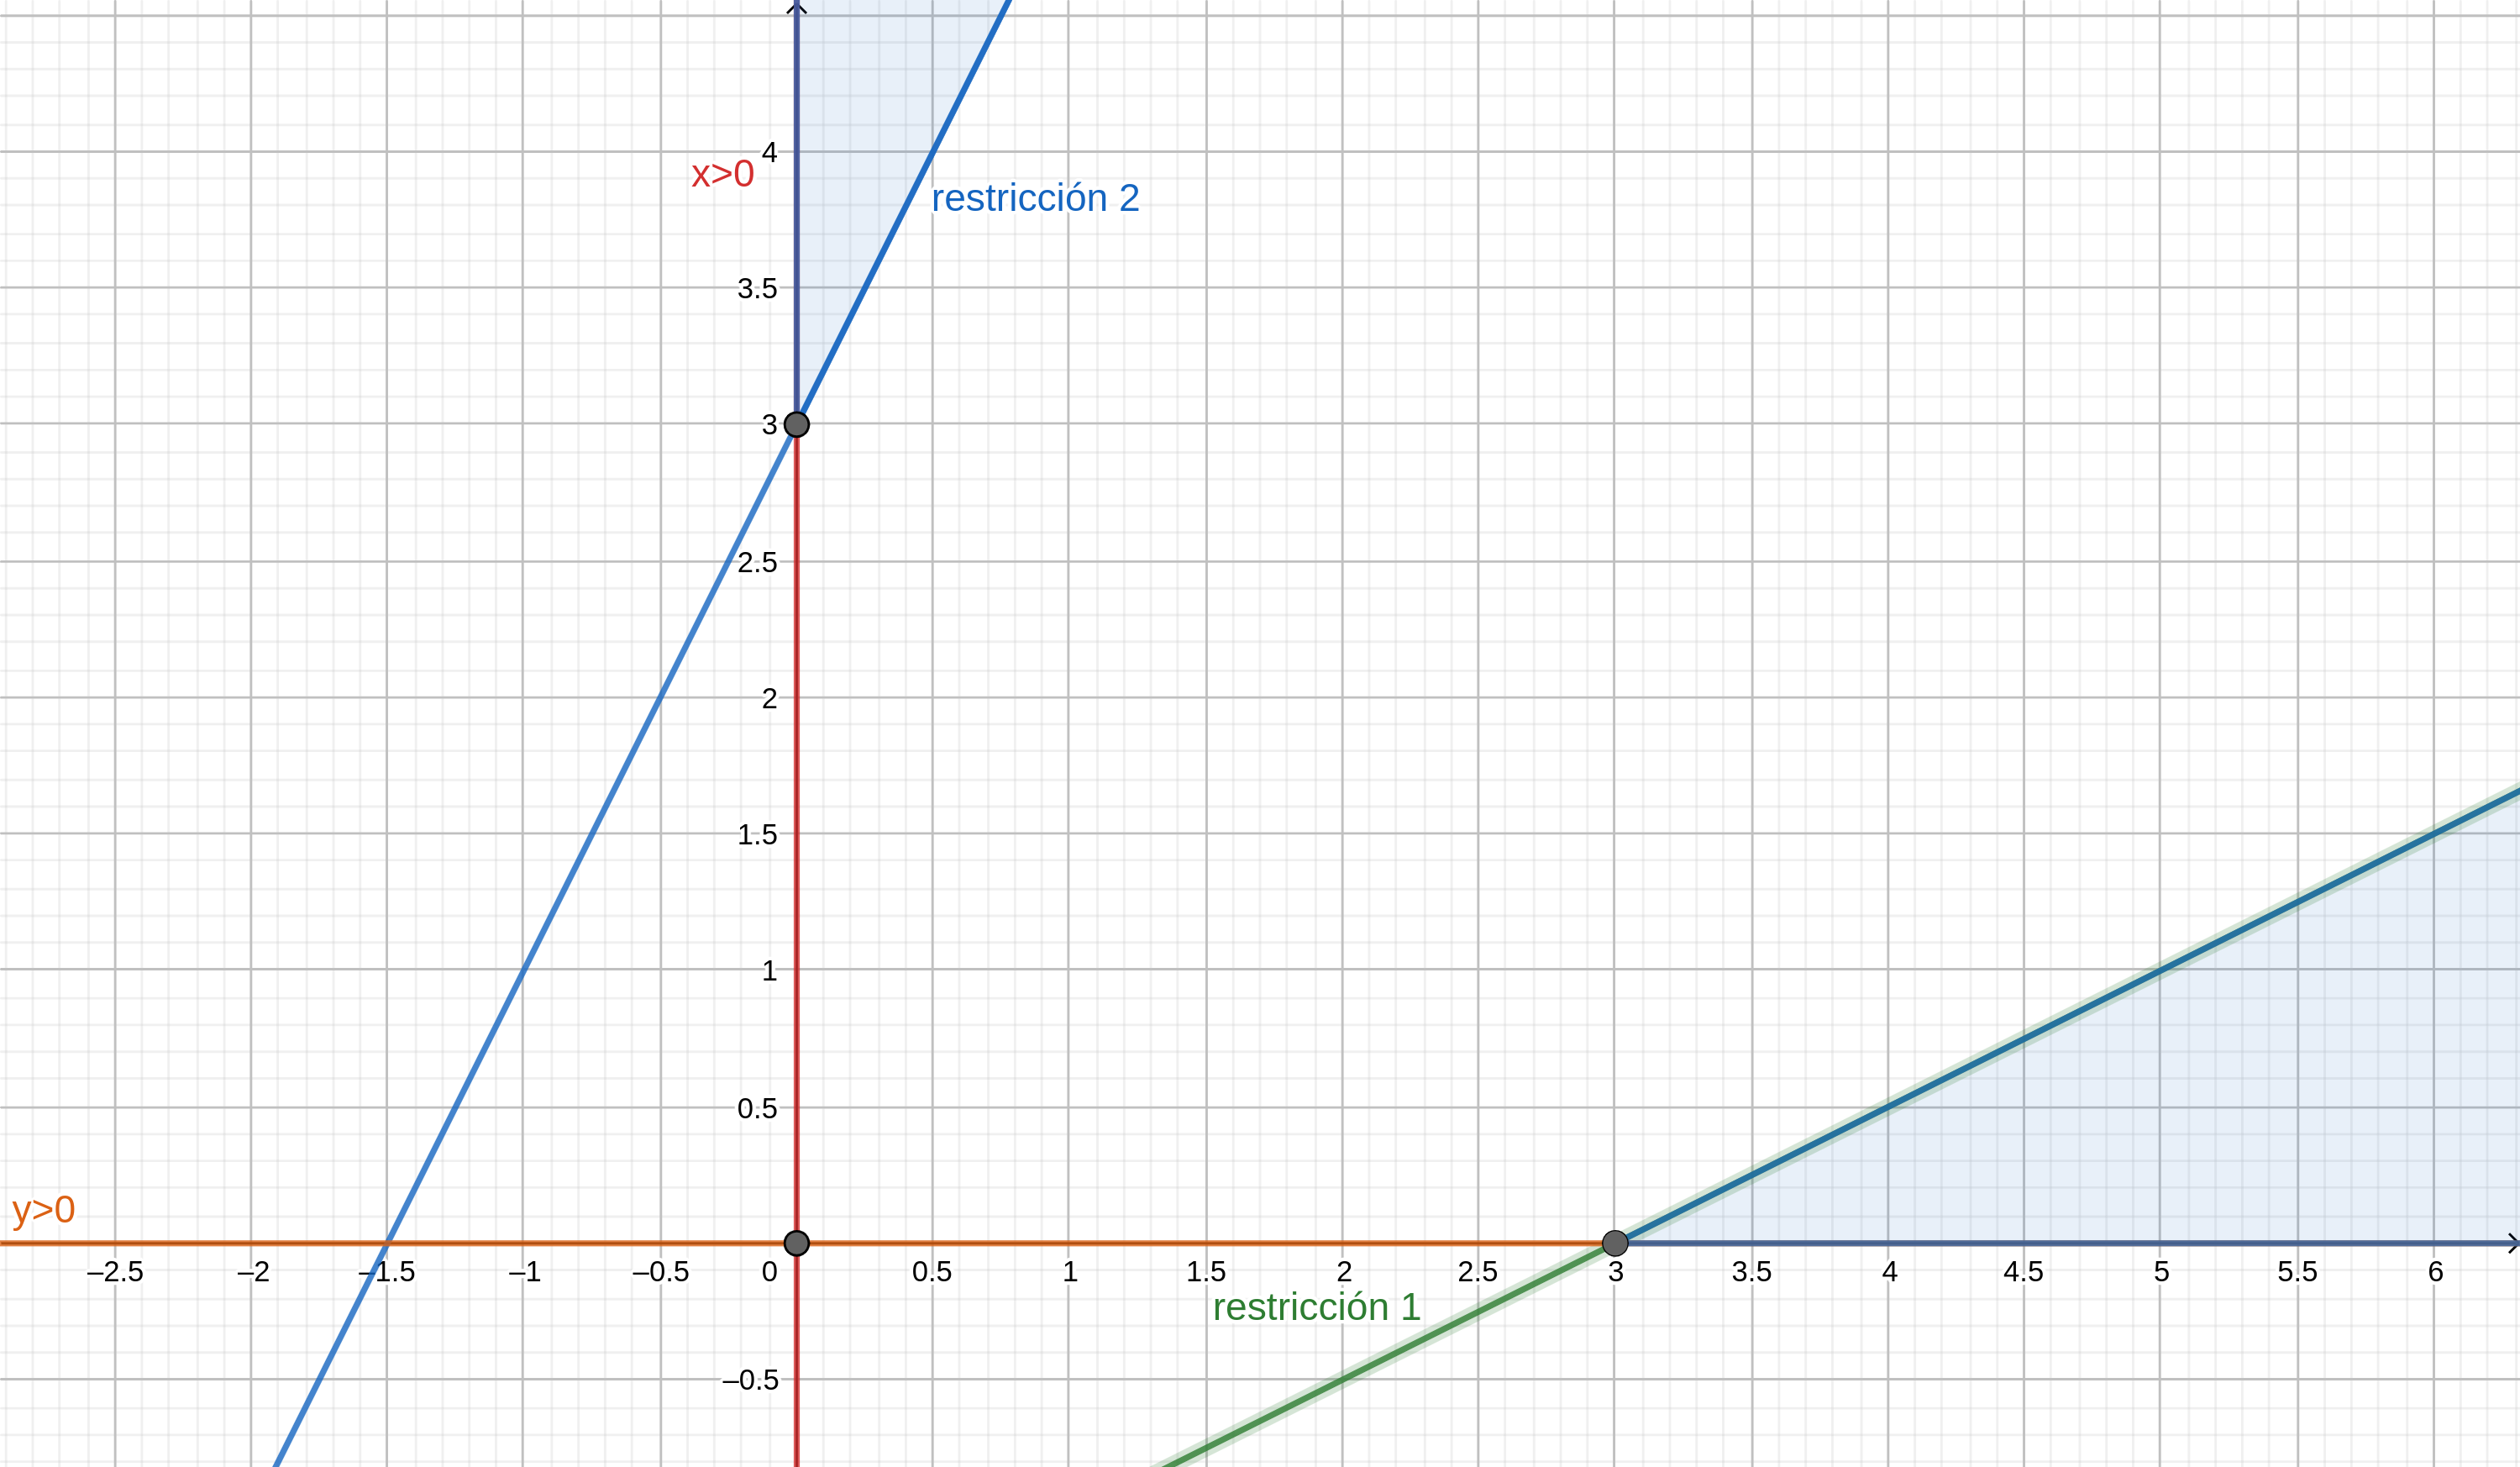
\includegraphics[scale=0.9]{ejercicio_4.png}
\caption{Representación grafica de las restricciones.}
\end{figure}

\item Considerar la relajación linel del problema 2. Encontrar el modelo dual y resolverlo con el método simplex dual.

\res Primero obtenermos el dual del problema 2, para ello ocupemos la definición \ref{d_dual}. Tenemos que 
\begin{align*}
c=\begin{pmatrix}
10 \\ 15\\ 4 \\2
\end{pmatrix} , \ \ A=\begin{pmatrix}
10 & 20 & 2 & 3 \\
5 & 5 & 5 & 4\\
4 & 2 & 6 & 6
\end{pmatrix} \ \ \ \text{y} \ \ \ b=\begin{pmatrix}
4000\\
1500\\
800
\end{pmatrix}.
\end{align*}
Por lo tanto, el problema dual sería
\begin{align*}
\min \ \ \ \ & w=4000y_1+1500y_2+800y_3\\
s.a:\ \ \ \ & 10y_1+5y_2+4y_3 \geq 10\\
	 & 20y_1+5y_2+2y_3 \geq 15\\
	 & 	2y_1+5y_2+6y_3 \geq 4\\
	 & 3y_1+4y_2+6y_3 \geq 2\\
	 &y_1,y_2, y_3 \geq 0
\end{align*}
Ahora hacemos ajustes:
\begin{align*}
\min \ \ \ \ & w-4000y_1-1500y_2-800y_3=0\\
s.a:\ \ \ \ & -10y_1-5y_2-4y_3 \leq -10\\
	 & -20y_1-5y_2-2y_3 \leq -15\\
	 & 	-2y_1-5y_2-6y_3 \leq -4\\
	 & -3y_1-4y_2-6y_3 \leq -2\\
	 &y_1,y_2, y_3 \geq 0.
\end{align*}
Después encontramos la forma aumentada agregando variables de holgura,
\begin{align*}
\min \ \ \ \ & w-4000y_1-1500y_2-800y_3=0\\
s.a:\ \ \ \ & -10y_1-5y_2-4y_3+y_4 =-10\\
	 & -20y_1-5y_2-2y_3+y_5 =-15\\
	 & 	-2y_1-5y_2-6y_3+y_6 = -4\\
	 & -3y_1-4y_2-6y_3 +y_7= -2\\
	 &y_1,y_2, y_3,y_4,y_5,y_6,y_7 \geq 0.
\end{align*}
Construimos la tabla \textit{Simplex}
\begin{equation}
\begin{array}{c}
\\
w \\
y_4\\
y_5 \\
y_6 \\
y_7 
\end{array}
\begin{bmatrix}
\begin{array}{c||cccccccc}
  w & y_1 & y_2 & y_3 & y_4 & y_5 & y_6 & y_7 & LD \\ \hline \hline
  1 &-4000 &-1500 &-800& 0 & 0 & 0 & 0 & 0\\ 
  0 & -10 & -5 & -4 & 1 & 0 & 0 & 0 & -10  \\
  0 & -20 & -5 & -2 & 0 & 1 & 0 & 0 & -15 \\
  0 &  -2 & -5 & -6 & 0 & 0 & 1 & 0 &  -4 \\
  0 &  -3 & -4 & -6 & 0 & 0 & 0 & 1 &  -2
\end{array}
\end{bmatrix}
\end{equation}
La variable que sale es $y_5$ ya que tiene el valor más negativo del lado derecho y la variable que entra es la que cumple $\min \left\{\frac{-4000}{-20}, \frac{-1500}{-5}, \frac{-800}{-2}\right\}=20$ la cual es la variable es $y_1$,
\begin{equation}
\begin{array}{c}
\\
w \\
y_4\\
y_1 \\
y_6 \\
y_7 
\end{array}
\begin{bmatrix}
\begin{array}{c||cccccccc}
  w & y_1 & y_2 & y_3 & y_4 & y_5 & y_6 & y_7 & LD \\ \hline \hline
  1 &-4000 &-1500 &-800& 0 & 0 & 0 & 0 & 0\\ 
  0 & -10 & -5 &-4 & 1 & 0 & 0 & 0 & -10  \\
  0 &   1 & 1/4&1/10 & 0 &-1/20 & 0 & 0 & 3/4 \\
  0 &  -2 & -5 & -6 & 0 & 0 & 1 & 0 &  -4 \\
  0 &  -3 & -4 & -6 & 0 & 0 & 0 & 1 &  -2
\end{array}
\end{bmatrix}
\end{equation}
Ahora realizamos operaciones básicas para eliminar la variable del resto de las filas.
\begin{equation}
\begin{array}{c}
\\
w \\
y_4\\
y_1 \\
y_6 \\
y_7 
\end{array}
\begin{bmatrix}
\begin{array}{c||cccccccc}
  w & y_1 & y_2 & y_3 & y_4 & y_5 & y_6 & y_7 & LD \\ \hline \hline
  1 & 0 &-500 &-400& 0 &-200 & 0 & 0 & 3000\\ 
  0 & 0 & -5/2 & -3 & 1 & -1/2 & 0 & 0 & -5/2  \\
  0 & 1 & 1/4& 1/10 & 0 &-1/20 & 0 & 0 & 3/4 \\
  0 & 0 & -9/2& -29/5 & 0 & -1/10 & 1 & 0 &  -5/2 \\
  0 & 0 & -13/4 & -57/10 & 0 & -3/20 & 0 & 1 &  1/4
\end{array}
\end{bmatrix}
\end{equation}
Ahora usando la prueba de optamilidad sebamos que aún no llegamos a ella, entonces la nueva variable que sale es $y_4$ y la variable que entra es la que cumple $\min \left\{\frac{500*2}{5}, \frac{400}{3} \right\}$ la cual es la variable es $y_3$,
\begin{equation}
\begin{array}{c}
\\
w \\
y_4\\
y_1 \\
y_6 \\
y_7 
\end{array}
\begin{bmatrix}
\begin{array}{c||cccccccc}
  w & y_1 & y_2 & y_3 & y_4 & y_5 & y_6 & y_7 & LD \\ \hline \hline
  1 & 0 &-500 &-400& 0 &-200 & 0 & 0 & 3000\\ 
  0 & 0 & 5/6 & 1 & -1/3 & 1/6 & 0 & 0 & 5/6  \\
  0 & 1 & 1/4& 1/10 & 0 &-1/20 & 0 & 0 & 3/4 \\
  0 & 0 & -9/2& -29/5 & 0 & -1/10 & 1 & 0 &  -5/2 \\
  0 & 0 & -13/4 & -57/10 & 0 & -3/20 & 0 & 1 &  1/4
\end{array}
\end{bmatrix}
\end{equation}
Ahora realizamos operaciones básicas para eliminar la variable del resto de las filas.
\begin{equation}
\begin{array}{c}
\\
w \\
y_3\\
y_1 \\
y_6 \\
y_7 
\end{array}
\begin{bmatrix}
\begin{array}{c||cccccccc}
  w & y_1 & y_2 & y_3 & y_4 & y_5 & y_6 & y_7 & LD \\ \hline \hline
  1 & 0 &-1000/6 & 0 & -400/3 &-800/6 & 0 & 0 & 20000/6\\ 
  0 & 0 & 5/6 & 1 & -1/3 & 1/6 & 0 & 0 & 5/6  \\
  0 & 1 & 1/6 & 0 & 1/30 &-1/15 & 0 & 0 & 40/60 \\
  0 & 0 & -10/30& 0 & -29/15 & 26/30 & 1 & 0 &  7/3 \\
  0 & 0 & 90/60 & 0 & -57/30 & 48/60 & 0 & 1 &  300/6
\end{array}
\end{bmatrix}
\end{equation}
Haciendo la prueba de optimalidad: todos los elementos de la última columa de la deracha son $\geq 0$, \textbf{por lo que podemos concluir que la solución optima es $y= \begin{pmatrix}
2/3& 0 & 5/6
\end{pmatrix}'$ con un valor en la función objetivo de $w=10000/3$.} Como observación podemos notar que se cumple el Teorema \ref{t_dual_debil}).

\section{Análisis de sensibilidad}
Considerar la relajación lineal del modelo del problema 2 en cada uno de los siguietnes incisos y concluir con la solución óptima del problema.

\item Determinar los rangos de variación (intervalos permisibles) en la utilidad unitaria de las variables no básicas de tal forma que la solución ótima no se altere.

\res Para obtener los intervalos permisibles tenemos que se debe de cumplir que $$c_j\leq y^*\bar{A}_j, \ \ j=1,2,3,4.$$
Del ejercicio 5 sabemos que la solución básica complenmentaría $y*$ en el problema dual es $y*= \begin{pmatrix}
2/3& 0 & 5/6
\end{pmatrix},$ y tenemos que $\bar{A}_1=\begin{pmatrix} 10 & 5 & 4\end{pmatrix}^T, \bar{A}_2=\begin{pmatrix}20 & 5 & 2\end{pmatrix}^T, \bar{A}_3=\begin{pmatrix} 2 & 5 & 6 \end{pmatrix}^T, \bar{A}_4=\begin{pmatrix} 3 & 4 & 6\end{pmatrix}^T.$ Entonces lo intervalos permisibles en la utilidad unitaria de las variables no básicas son, para $c_1$
\begin{align*}
c_1\leq y^*\bar{A}_1 = \begin{pmatrix}
2/3& 0 & 5/6
\end{pmatrix}\begin{pmatrix} 10 \\
5 \\
4
\end{pmatrix}=\frac{40+20}{6}=10\ \ \bf \Rightarrow c_1\leq 10,\\
c_2\leq y^*\bar{A}_2 = \begin{pmatrix}
2/3& 0 & 5/6
\end{pmatrix}\begin{pmatrix} 20 \\
5 \\
2
\end{pmatrix}=\frac{80+10}{6}=15\ \ \bf \Rightarrow c_2\leq 15\\
c_3\leq y^*\bar{A}_3 = \begin{pmatrix}
2/3& 0 & 5/6
\end{pmatrix}\begin{pmatrix} 2 \\
5 \\
6
\end{pmatrix}=\frac{8+30}{6}=19/3\ \ \bf \Rightarrow c_3\leq 19/3, \ \ \text{y}\\
c_4\leq y^*\bar{A}_4 = \begin{pmatrix}
2/3& 0 & 5/6
\end{pmatrix}\begin{pmatrix} 3 \\
4 \\
6
\end{pmatrix}=\frac{12+30}{6}=7\ \ \bf \Rightarrow c_4\leq 7. \ \ \finf
\end{align*}


\item Evaluar el efecto de un cambio en la utilidad del producto tres de $\$4$ a $\$5$ (sin utilizar la información de los rangos de variación.

\res El problema original es 
\begin{align*}
\max\ \ \ \ & z=10x_1+15x_2+4x_3+2x_4.\\
s.a:\ \ \ \ & 10x_1+20x_2 +2x_3+3x_4\leq 4000\\
	 & 5x_1+5x_2+5x_3+4x_4\leq 1500\\
	 & 4x_1+2x_2+6x_3+6x_4 \leq 800\\
	 & x_1,x_2,x_3,x_4 \geq 0. 
\end{align*}
Y la solución básica complenmentaría $y*$ en el problema dual es $y*= \begin{pmatrix}
2/3& 0 & 5/6
\end{pmatrix}$. Entonces, considerando el cambio en $c_3=5$ el problema con cambios sería
\begin{align*}
\max\ \ \ \ & z=10x_1+15x_2+5x_3+2x_4\\
s.a:\ \ \ \ & 10x_1+20x_2 +2x_3+3x_4\leq 4000\\
	 & 5x_1+5x_2+5x_3+4x_4\leq 1500\\
	 & 4x_1+2x_2+6x_3+6x_4 \leq 800\\
	 & x_1,x_2,x_3,x_4 \geq 0. 
\end{align*}
Como el cambio solo se realizó en $x_3$, entonces encontramos la restricción dual asociada a esa columna donde se realizaron los cambios
$$2y_1+5y_2+6y_3\geq 5.$$
Sustiyendo los valores de la solución óptima tenemos que 
\begin{align*}
2(2/3)+5(0)+6(5/6)\geq 5\\
19/3\approx 6.333\geq 5.
\end{align*}
Por lo tanto, \textbf{como se satisface la restricción dual implica que la solución óptima del modelo original sigue siendo válida} \ \ \ \ \fin
Si observamos los rangos permisibles se satisfacen lo que se obtuvo.

\item Evaluar los posibles efectos en la solución óptima al realizar el siguiente cambio $a_3= \begin{pmatrix}
2 & 3 & 1
\end{pmatrix}^T$.

\res Tenemos que el problema con el cambio es 
\begin{align*}
\max\ \ \ \ & z=10x_1+15x_2+4x_3+2x_4.\\
s.a:\ \ \ \ & 10x_1+20x_2 +2x_3+3x_4\leq 4000\\
	 & 5x_1+5x_2+3x_3+4x_4\leq 1500\\
	 & 4x_1+2x_2+6x_3+6x_4 \leq 800\\
	 & x_1,x_2,x_3,x_4 \geq 0. 
\end{align*}
La restricción dual asociada a $x_3$ en el problema con los cambios es
\begin{align*}
2y_1+3y_2+y_3\geq 4
\end{align*}
Y la solución complementaria, es decir, la solución del problema dual del problema original es $y^*\begin{pmatrix}
2/3 & 0 & 5/6
\end{pmatrix}$, entonces verifiquemos si la restricción dual asociada a $x_3$ sea válida con solución dual
\begin{align*}
2y_1+3y_2+y_3\geq 4\\
2(2/3)+3(0)+1(5/6)\geq 4\\
13/6\approx2.166\geq 4.
\end{align*}
\textbf{Como la desigualdad no se cumple, entonces la solución actual ya no es óptima.} Por lo que hay reoptimizar nuevamente, primero actualizamos los valores en la tabla óptima original. Primero encontremos los siguientes valores
\begin{align*}
z_j^* -\bar{c}_j=y^*\bar{A}_j-\bar{c}_j\\
A^*_j=S^*\bar{A}_j.
\end{align*}
Como los cambios se hicieron en $x_3$ entonces $j=3$, y de la tabla dual tenemos que $\bar{A}_3=\begin{pmatrix}
2\\
3\\
1
\end{pmatrix}, S^*=\begin{pmatrix}
1/15 & 0 & -1/6\\
-1/6 & 1 & -5/6\\
-1/30 & 0 & 1/3
\end{pmatrix} $ (Ver la Tabla \ref{t_optima_original}). 
\begin{align*}
z_3^* -\bar{c}_3=y^*\bar{A}_j-\bar{c}_3=\begin{pmatrix}
2/3 & 0 & 5/6
\end{pmatrix}\begin{pmatrix}
2\\
3\\
1
\end{pmatrix}-4=-\frac{11}{6},\\
A^*_3 = \begin{pmatrix}
1/15 & 0 & -1/6\\
-1/6 & 1 & -5/6\\
-1/30 & 0 & 1/3
\end{pmatrix}\begin{pmatrix}
2\\
3\\
1
\end{pmatrix}=\begin{pmatrix}
-1/30\\
11/6\\
8/30
\end{pmatrix}
\end{align*}
Sustituimos estos varoles en la tabla óptima del problema original (Tabla \ref{t_optima_original}) y reoptimizamos con simples. La tabla óptima es:
\begin{equation} 
\begin{array}{c}
\\
z \\ 
x_2 \\
x_6 \\
x_1
\end{array}
\begin{bmatrix}
\begin{array}{c||cccccccc}
  z & x_1 & x_2 & x_3 & x_4 & x_5 & x_6 & x_7 & LD\\ \hline \hline
  1 & 0 & 0 & 7/3 & 5 & 2/3 & 0 & 5/6 & 10000/3\\ 
  0 & 0 & 1 &-13/15 & -4/5 & 1/15 & 0 &-1/6 & 400/3  \\
  0 & 0 & 0 &-1/3 & -3/2 & -1/6 & 1 & -5/6& 500/3 \\
  0 & 1 & 0 & 29/15 & 19/10 & -1/30 & 0 & 1/3 & 400/3 \\
\end{array}
\end{bmatrix}
\end{equation}
Sustituimos:
\begin{equation} 
\begin{array}{c}
\\
z \\ 
x_2 \\
x_6 \\
x_1
\end{array}
\begin{bmatrix}
\begin{array}{c||cccccccc}
  z & x_1 & x_2 & x_3 & x_4 & x_5 & x_6 & x_7 & LD\\ \hline \hline
  1 & 0 & 0 &-11/6 & 5 & 2/3 & 0 & 5/6 & 10000/3\\ 
  0 & 0 & 1 &-1/30 & -4/5 & 1/15 & 0 &-1/6 & 400/3  \\
  0 & 0 & 0 &11/6  & -3/2 & -1/6 & 1 & -5/6& 500/3 \\
  0 & 1 & 0 & 8/30 & 19/10 & -1/30 & 0 & 1/3 & 400/3 \\
\end{array}
\end{bmatrix}
\end{equation}
En la tabla anterior vemos claramente que no es óptima, por lo que la nueva variable que entra es $x_3$ y la variable es la que cumple $\min \left\{4000, \frac{500*6}{33},\frac{4000}{8} \right\}$, la cual es la variable es $x_6$,
\begin{equation} 
\begin{array}{c}
\\
z \\ 
x_2 \\
x_3 \\
x_1
\end{array}
\begin{bmatrix}
\begin{array}{c||cccccccc}
  z & x_1 & x_2 & x_3 & x_4 & x_5 & x_6 & x_7 & LD\\ \hline \hline
  1 & 0 & 0 &-11/6 & 5 & 2/3 & 0 & 5/6 & 10000/3\\ 
  0 & 0 & 1 &-1/30 & -4/5 & 1/15 & 0 &-1/6 & 400/3  \\
  0 & 0 & 0 & 1  & -9/11 & -1/11 & 6/11 & -5/11& 1000/11 \\
  0 & 1 & 0 & 8/30 & 19/10 & -1/30 & 0 & 1/3 & 400/3 \\
\end{array}
\end{bmatrix}
\end{equation}
Sustituimos:
\begin{equation} 
\begin{array}{c}
\\
z \\ 
x_2 \\
x_3 \\
x_1
\end{array}
\begin{bmatrix}
\begin{array}{c||cccccccc}
  z & x_1 & x_2 & x_3 & x_4 & x_5 & x_6 & x_7 & LD\\ \hline \hline
  1 & 0 & 0 & 0 &7/2 & 1/2 & 1 & 0 & 10500/3\\ 
  0 & 0 & 1 & 0 & -91/110 & 7/110 & 1/55 &-2/11 & 4500/33  \\
  0 & 0 & 0 & 1 & -9/11 & -1/11 & 6/11 & -5/11& 1000/11 \\
  0 & 1 & 0 & 0 & 221/11 & -1/66 & -4/55 & 59/165 & 3600/33 \\
\end{array}
\end{bmatrix}
\end{equation}
Haciendo la prueba de optimalidad: todos los elementos de la primera fila son $\geq 0$, \textbf{por lo que podemos concluir que la solución optima con la modificación es $x_{new}^*= \begin{pmatrix}
1200/11& 1500/11 & 1000/11
\end{pmatrix}'$ con un valor en la función objetivo de $z=10500/3=3500$.}




\item El tomador de decisiones está estudiando la posibilidad de adicionar un nuevo artículo a su línea de productos actuales con coeficientes 12 en la función objetivo y en las restricciones con coeficientes 9, 7 y 6 respectivamente. ¿Si es recomendable esta acción?

\res Denotemos a $x_n$ a la variable del nuevo artículo, entonces los parámetros asociados a la nueva variable son 
\begin{align*}
c_n=0, \ \ \ A_n=\begin{pmatrix}
0\\
0\\
0
\end{pmatrix} \ \ \ \Rightarrow \bar{c}_n = 12, \ \ \text{y} \ \ \bar{A}_n=\begin{pmatrix}
9\\
7\\
6
\end{pmatrix}.
\end{align*}
Entonces el problema con cambios es 
\begin{align*}
\max\ \ \ \ & z=10x_1+15x_2+4x_3+2x_4+12x_n.\\
s.a:\ \ \ \ & 10x_1+20x_2 +2x_3+3x_4+9x_n\leq 4000\\
	 & 5x_1+5x_2+5x_3+4x_4+7x_n\leq 1500\\
	 & 4x_1+2x_2+6x_3+6x_4+6x_n \leq 800\\
	 & x_1,x_2,x_3,x_4,x_n \geq 0. 
\end{align*}
La restricción dual asociada a $x_n$ en el problema con los cambios es $$9y_1+7y_2+6y_3\geq 12.$$
Y tenemos que la solución complementarioa, es decir, la solución del problema dual del problema original es $y^*=\begin{pmatrix}
2/3 & 0 & 5/6
\end{pmatrix}$. Verifiquemos si la restricción dual asociada a $x_n$ sigue siendo válida con solución dual
\begin{align*}
9y_1+7y_2+6y_3\geq 12\\
9(2/3)+7(0)+6(5/6)\geq 12\\
11 \geq 12.
\end{align*}
Vemos que la desigualdad no se cumple, \textbf{por lo que agregar agregar un nuevo artículo hace inválida la solución óptima de modelo por lo que no sería recomendable o si se ingresa se tendría que encontrar la solución óptima nuevamente.}  Por lo que hay reoptimizar nuevamente, primero actualizamos los valores en la tabla óptima original. Primero encontremos los siguientes valores
\begin{align*}
z_j^* -\bar{c}_j=y^*\bar{A}_j-\bar{c}_j\\
A^*_j=S^*\bar{A}_j.
\end{align*}
Como los cambios se hicieron en $x_n$ entonces $j=n$, y de la tabla dual tenemos que $\bar{A}_n=\begin{pmatrix}
9\\
7\\
6
\end{pmatrix}, S^*=\begin{pmatrix}
1/15 & 0 & -1/6\\
-1/6 & 1 & -5/6\\
-1/30 & 0 & 1/3
\end{pmatrix} $ (Ver la Tabla \ref{t_optima_original}). 
\begin{align*}
z_n^* -\bar{c}_n=y^*\bar{A}_n-\bar{c}_n=\begin{pmatrix}
2/3 & 0 & 5/6
\end{pmatrix}\begin{pmatrix}
9\\
7\\
6
\end{pmatrix}-12=-1,\\
A^*_3 = \begin{pmatrix}
1/15 & 0 & -1/6\\
-1/6 & 1 & -5/6\\
-1/30 & 0 & 1/3
\end{pmatrix}\begin{pmatrix}
9\\
7\\
6
\end{pmatrix}=\begin{pmatrix}
-2/5\\
1/2\\
17/10
\end{pmatrix}
\end{align*}
Sustituimos estos varoles en la tabla óptima del problema original (Tabla \ref{t_optima_original}) y reoptimizamos con simples. La tabla óptima es:
\begin{equation} 
\begin{array}{c}
\\
z \\ 
x_2 \\
x_6 \\
x_1
\end{array}
\begin{bmatrix}
\begin{array}{c||cccccccc}
  z & x_1 & x_2 & x_3 & x_4 & x_5 & x_6 & x_7 & LD\\ \hline \hline
  1 & 0 & 0 & 7/3 & 5 & 2/3 & 0 & 5/6 & 10000/3\\ 
  0 & 0 & 1 &-13/15 & -4/5 & 1/15 & 0 &-1/6 & 400/3  \\
  0 & 0 & 0 &-1/3 & -3/2 & -1/6 & 1 & -5/6& 500/3 \\
  0 & 1 & 0 & 29/15 & 19/10 & -1/30 & 0 & 1/3 & 400/3 \\
\end{array}
\end{bmatrix}
\end{equation}
Sustituimos:
\begin{equation} 
\begin{array}{c}
\\
z \\ 
x_2 \\
x_6 \\
x_1
\end{array}
\begin{bmatrix}
\begin{array}{c||ccccccccc}
  z & x_1 & x_2 & x_3 & x_4 & x_5 & x_6 & x_7 & x_n& LD\\ \hline \hline
  1 & 0 & 0 & 7/3 & 5 & 2/3 & 0 & 5/6 & -1 & 10000/3\\ 
  0 & 0 & 1 &-13/15 & -4/5 & 1/15 & 0 &-1/6& -2/5 & 400/3  \\
  0 & 0 & 0 &-1/3 & -3/2 & -1/6 & 1 & -5/6&1/2& 500/3 \\
  0 & 1 & 0 & 29/15 & 19/10 & -1/30 & 0 & 1/3 &17/10&400/3
\end{array}
\end{bmatrix}
\end{equation}
En la tabla anterior vemos claramente que no es óptima, por lo que la nueva variable que entra es $x_n$ y la variable es la que cumple $\min \left\{\frac{400*5}{6}, \frac{500*2}{3},\frac{4000}{21} \right\}$, la cual es la variable es $x_1$,
\begin{equation} 
\begin{array}{c}
\\
z \\ 
x_2 \\
x_6\\
x_1
\end{array}
\begin{bmatrix}
\begin{array}{c||ccccccccc}
  z & x_1 & x_2 & x_3 & x_4 & x_5 & x_6 & x_7 & x_n& LD\\ \hline \hline
  1 & 0 & 0 & 7/3 & 5 & 2/3 & 0 & 5/6 & -1 & 10000/3\\ 
  0 & 0 & 1 &-13/15 & -4/5 & 1/15 & 0 &-1/6& -2/5 & 400/3  \\
  0 & 0 & 0 &-1/3 & -3/2 & -1/6 & 1 & -5/6&1/2& 500/3 \\
  0 & 1 & 0 & 58/85 & 19/17 & -1/51 & 0 &17/51 &1&4000/51
\end{array}
\end{bmatrix}
\end{equation}
Hacemos la variable $x_n$ en su forma cánonica
\begin{equation} 
\begin{array}{c}
\\
z \\ 
x_2 \\
x_6\\
x_n
\end{array}
\begin{bmatrix}
\begin{array}{c||ccccccccc}
  z & x_1 & x_2 & x_3 & x_4 & x_5 & x_6 & x_7 & x_n& LD\\ \hline \hline
  1 & 0 & 0 & 769/255 & 104/17 & 11/17 & 0 & 7/6 &0& 58000/17\\ 
  0 & 0 & 1 &-757/1275 & -6/17 & 1/17 & 0 &-1/30&0& 2800/17   \\
  0 & 0 & 0 &-172/255& -35/17& -8/51& 1 &-1&0& 6500/51 \\
  0 & 1 & 0 & 58/85 & 19/17 & -1/51 & 0 &17/51 &1&4000/51
\end{array}
\end{bmatrix}
\end{equation}
Haciendo la prueba de optimalidad: todos los elementos de la primera fila son $\geq 0$, \textbf{por lo que podemos concluir que la solución optima con la modificación es $x_{new}^*= \begin{pmatrix}
0 & 2800/17 & 0 & 4000/51
\end{pmatrix}'$ con un valor en la función objetivo de $z_{new}^*=58000/17$.} Si comparamos el valor de la función objetivo del problema sin el producto nuevo y agregandolo notamos que hay un diferencia de $\frac{1000}{3}-\frac{58000}{17}=-78.43,$ \textbf{este significa que aumento el valor objetivo agregando el nuevo producto, por lo que si sería recomendable.} \ \ \ \ \fin


\item El tomador de decisiones ahora quiere tomar en cuenta en el model una restricción de demanda mínima para mantener una cierta porción en el mercado, la cual representa una nueva restricción: 
$$x_1+2x_2+3x_3+4x_4 \geq 500.$$
Evaluar los efectos de incluir la nueva restricción.

\res El modelo con la nueva restricción sería 
\begin{align*}
\max\ \ \ \ & z=10x_1+15x_2+4x_3+2x_4.\\
s.a:\ \ \ \ & 10x_1+20x_2 +2x_3+3x_4\leq 4000\\
	 & 5x_1+5x_2+5x_3+4x_4\leq 1500\\
	 & 4x_1+2x_2+6x_3+6x_4 \leq 800\\
	 & x_1+ 2x_2+3x_3+4x_4 \geq 500\\
	 & x_1,x_2,x_3,x_4 \geq 0. 
\end{align*}
La solución óptima del modelo original es $x^*=\begin{pmatrix}
400/3 & 400/3 & 0 & 0
\end{pmatrix}.$ Verifiquemos si la solución óptima actual satisface la nueva restricción
\begin{align*}
x_1+ 2x_2+3x_3+4x_4 \geq 500\\
400/3+2(400/3)+3(0)+4(0)\geq 500\\
1200/3=400 \geq 500.
\end{align*}
Entonces, \textbf{como no se satisface la nueva restricción, entonces la solución actual ya no es valida}. Entonces debemos encontrar la forma aumentada de esta nueva restricción:
\begin{align*}
x_1+ 2x_2+3x_3+4x_4 \geq 500\\
-x_1- 2x_2-3x_3-4x_4 \leq-500\\
-x_1- 2x_2-3x_3-4x_4+x_8 =-500
\end{align*}
Por lo tanto, ahora introducimos un renglón adicional a la tabla final del método simplex del problema original (Tabla \ref{t_optima_original}) para introducir la nueva restricción, y también hay que agregar una nueva columna considerando la nueva variable de holgura (la que corresponde a la restricción nueva) como parte de la base La tabla final del problema original es:
\begin{equation} 
\begin{array}{c}
\\
z \\ 
x_2 \\
x_6 \\
x_1
\end{array}
\begin{bmatrix}
\begin{array}{c||cccccccc}
  z & x_1 & x_2 & x_3 & x_4 & x_5 & x_6 & x_7 & LD\\ \hline \hline
  1 & 0 & 0 & 7/3 & 5 & 2/3 & 0 & 5/6 & 10000/3\\ 
  0 & 0 & 1 &-13/15 & -4/5 & 1/15 & 0 &-1/6 & 400/3  \\
  0 & 0 & 0 &-1/3 & -3/2 & -1/6 & 1 & -5/6& 500/3 \\
  0 & 1 & 0 & 29/15 & 19/10 & -1/30 & 0 & 1/3 & 400/3 \\
\end{array}
\end{bmatrix}
\end{equation}
La nueva tabla es
\begin{equation} 
\begin{array}{c}
\\
z \\ 
x_2 \\
x_6 \\
x_1\\
x_8
\end{array}
\begin{bmatrix}
\begin{array}{c||ccccccccc}
  z & x_1 & x_2 & x_3 & x_4 & x_5 & x_6 & x_7 & x_8 & LD\\ \hline \hline
  1 & 0 & 0 & 7/3 & 5 & 2/3 & 0 & 5/6 &0 & 10000/3\\ 
  0 & 0 & 1 &-13/15 & -4/5 & 1/15 & 0 &-1/6 &0& 400/3  \\
  0 & 0 & 0 &-1/3 & -3/2 & -1/6 & 1 & -5/6&0& 500/3 \\
  0 & 1 & 0 & 29/15 & 19/10 & -1/30 & 0 & 1/3 &0&400/3 \\
    0 & -1 & -2 & -3 & -4 & 0 & 0 & 0 &1&-500
\end{array}
\end{bmatrix}
\end{equation}
Debemos asegurarnos que las variables básicas tengan forma canónica, en este caso hay que regresarle la forma canónica a $x_1$ y $x_2$, primero lo hacemos para $x_1$
\begin{equation} 
\begin{array}{c}
\\
z \\ 
x_2 \\
x_6 \\
x_1\\
x_8
\end{array}
\begin{bmatrix}
\begin{array}{c||ccccccccc}
  z & x_1 & x_2 & x_3 & x_4 & x_5 & x_6 & x_7 & x_8 & LD\\ \hline \hline
  1 & 0 & 0 & 7/3 & 5 & 2/3 & 0 & 5/6 &0 & 10000/3\\ 
  0 & 0 & 1 &-13/15 & -4/5 & 1/15 & 0 &-1/6 &0& 400/3  \\
  0 & 0 & 0 &-1/3 & -3/2 & -1/6 & 1 & -5/6&0& 500/3 \\
  0 & 1 & 0 & 29/15 & 19/10 & -1/30 & 0 & 1/3 &0&400/3 \\
  0 & 0 & -2 &-16/15 & -21/10 &-1/30 & 0 & 1/3 &1&-1100/3
\end{array}
\end{bmatrix}
\end{equation}
ahora para $x_2$
\begin{equation} 
\begin{array}{c}
\\
z \\ 
x_2 \\
x_6 \\
x_1\\
x_8
\end{array}
\begin{bmatrix}
\begin{array}{c||ccccccccc}
  z & x_1 & x_2 & x_3 & x_4 & x_5 & x_6 & x_7 & x_8 & LD\\ \hline \hline
  1 & 0 & 0 & 7/3 & 5 & 2/3 & 0 & 5/6 &0 & 10000/3\\ 
  0 & 0 & 1 &-13/15 & -4/5 & 1/15 & 0 &-1/6 &0& 400/3  \\
  0 & 0 & 0 &-1/3 & -3/2 & -1/6 & 1 & -5/6&0& 500/3 \\
  0 & 1 & 0 & 29/15 & 19/10 & -1/30 & 0 & 1/3 &0&400/3 \\
  0 & 0 & 0 &-14/5 & -37/10 &1/10 & 0 & 0 &1&-100
\end{array}
\end{bmatrix}
\end{equation}
Ahora observamos que existe un elemento en la última columna de la derecha con valor negativo, por lo que debemos reoptimizar utilizando el método simplex dual. La nueva variable que entra es $x_3$ y la variable es la que cumple $\min \left\{\frac{7*5}{14*3}, \frac{50}{37},\frac{20}{3} \right\}$, la cual es la variable es $x_3$,
\begin{equation} 
\begin{array}{c}
\\
z \\ 
x_2 \\
x_6 \\
x_1\\
x_3
\end{array}
\begin{bmatrix}
\begin{array}{c||ccccccccc}
  z & x_1 & x_2 & x_3 & x_4 & x_5 & x_6 & x_7 & x_8 & LD\\ \hline \hline
  1 & 0 & 0 & 7/3 & 5 & 2/3 & 0 & 5/6 &0 & 10000/3\\ 
  0 & 0 & 1 &-13/15 & -4/5 & 1/15 & 0 &-1/6 &0& 400/3  \\
  0 & 0 & 0 &-1/3 & -3/2 & -1/6 & 1 & -5/6&0& 500/3 \\
  0 & 1 & 0 & 29/15 & 19/10 & -1/30 & 0 & 1/3 &0&400/3 \\
  0 & 0 & 0 & 1 & 37/28 &-1/28& 0 & 0 & -5/14&250/7
\end{array}
\end{bmatrix}
\end{equation}
Sustituimos:
\begin{equation} 
\begin{array}{c}
\\
z \\ 
x_2 \\
x_6 \\
x_1\\
x_3
\end{array}
\begin{bmatrix}
\begin{array}{c||ccccccccc}
  z & x_1 & x_2 & x_3 & x_4 & x_5 & x_6 & x_7 & x_8 & LD\\ \hline \hline
  1 & 0 & 0 &0& 23/12 & 3/4&0&5/6&5/6 &9750/3\\ 
  0 & 0 & 1 &0& 29/84 & 1/28& 0 &-1/6 &-13/42&1150/7  \\
  0 & 0 & 0 &0&-89/84&-5/28& 1 & -5/6&-5/42&1250/7 \\
  0 & 1 & 0 &0&-55/84 & 1/28 & 0 &1/3&29/42&450/7 \\
  0 & 0 & 0 & 1 & 37/28 &-1/28& 0 & 0 & -5/14&250/7
\end{array}
\end{bmatrix}
\end{equation}
Haciendo la prueba de optimalidad: todos los elementos de la primera fila son $\geq 0$, \textbf{por lo que podemos concluir que la solución optima con la modificación es $$x_{new}^*= \begin{pmatrix}
450/7&1150/7 &250/7&0
\end{pmatrix}'$$ con un valor en la función objetivo de $z_{new}^*=9750/3=3250$} \ \ \ \fin



\end{enumerate}

\end{document}